\documentclass[a4paper,11pt]{article}
\usepackage[american]{babel}
\usepackage[utf8]{inputenc}
\usepackage{geometry}

\usepackage{booktabs}  
\usepackage{graphicx} 
\usepackage{listings}
\lstset{%
backgroundcolor=\color{cyan!10},
basicstyle=\ttfamily,
numbers=left,numberstyle=\scriptsize
}

\usepackage[wby]{callouts}

\title{COP290 - Case Study I - Electronic Voting Machines}
\author{N. Akash \\ \href{iakash2702@gmail.com}}

\begin{document}

\maketitle

\section{Introduction}
India is the largest democracy in the world and hence has to hold the largest elections in the world. With a voting population in the 9th order of magnitude this is no easy task. And it is not made easier by the fact that people contesting the elections generally will do whatever it takes to win, including tampering the election results in their favor. Elections lie at the heart of the Indian Democracy and hence they need to be held with fool proof security and integrity. This also means protecting the individual voter. Hence ensuring anonymity is also very crucial. Since a large number of Indian voters are illiterate or not familiar with technology, the voting process should be as simple as possible to reduce the chance of casting a wrong vote too. 

Electronic Voting Machines are very simple, easy to use, light weight, portable, battery run devices. They also help in saving a lot of ballot paper. The also very cost efficient. However EVM's have been facing rising opposition despite these advantages. This is mainly because of the fact that EVM's are being claimed to be tamper-able.  

This paper investigates (to the best of the author's abilities) the existing technology being used in the EVM's and its pitfalls. Some suggestions to improve it have also been made.


\section{Existing Model}
The existing model has 2 main units. The control unit and the ballot unit. They are both connected by a 5 meter long wire. In some versions (VVPAT, to be specific), there is also another printer unit attached to the ballot unit as an extra layer of authentication. 

\subsection{Ballot Unit}
The ballot unit is the device which the voters will be using to cast their vote. It has 16 buttons with each button having the capacity to hold 4 people. That is achieved using a slider switch which assumes one of 4 positions. The voter presses the button corresponding to their choice of candidate and registers their vote. This vote is stored in the Control Unit. Only the first key press is registered and immediately after that the Control Unit locks the Ballot Unit. No further votes can be cast until the Ballot Unit is unlocked. 

The ballot unit has an array of electronically programmable logic devices or ELPD's. Each one acts as a switch which when triggered by the press of a ballot casts a vote and consequentially is then locked. It is unlocked only after getting the signal from the control unit. 

\begin{figure}[h!]
  \centering
  \begin{annotate}{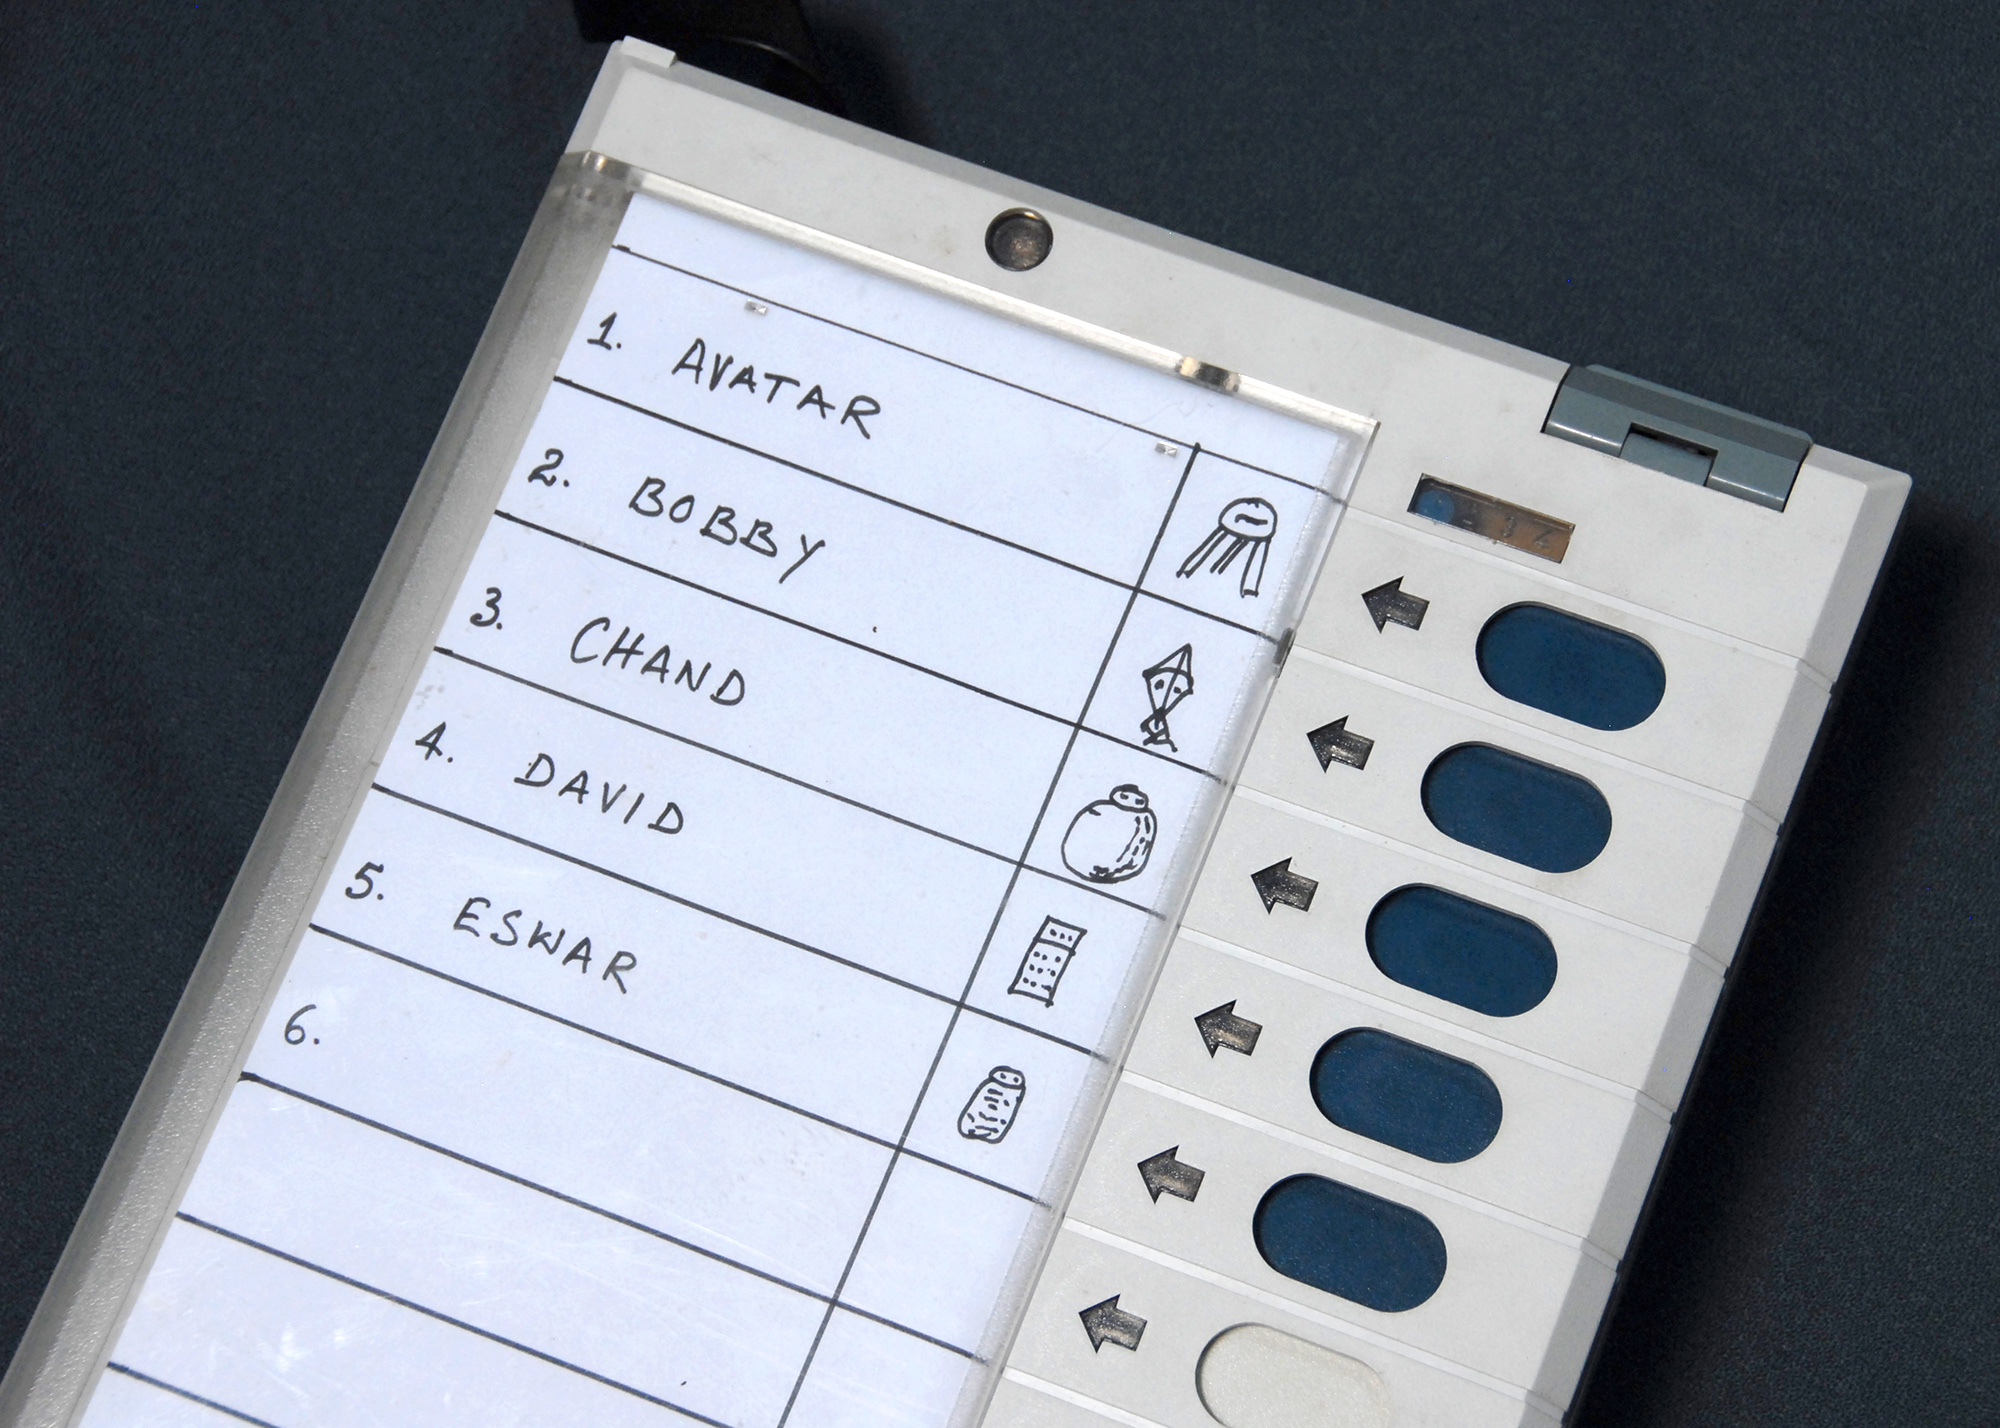
\includegraphics[width=0.7\textwidth]{ballot.jpg}}{0.7}
  \end{annotate}
  \caption{Ballot Unit\protect\footnotemark}\label{fig:Airbus}
\end{figure}


\subsection{Control Unit}
The Control Unit will be with the Presiding Officer or some other government agent at the polling station. The ballot unit can be unlocked only when they press the ballot button. So the presiding officer needs to ensure that each person is voting only once. This is done by applying indelible ink on each person who has voted so that they can be stopped from casting multiple votes. The control unit has 2 more important buttons other than the ballot button, the end button and the result button. The end button is pressed at the end of the election process for the day. It is then sealed and taken to a strong room where it is kept till the day of counting. On that day the result button is pressed. That specific button is sealed and it is ensured that the seal is not broken till the day of counting the votes. On pressing the result button the LCD screen shows the votes obtained by each candidate on the ballot. They are noted down and added. 

To be precise the Control Unit has EEPROM chips which allow non volatile storage of data. And the CPU is a non re-programmable non readable chip called the Renesas H8/3644 micro-controller. 

\begin{figure}[h!]
  \centering
  \begin{annotate}{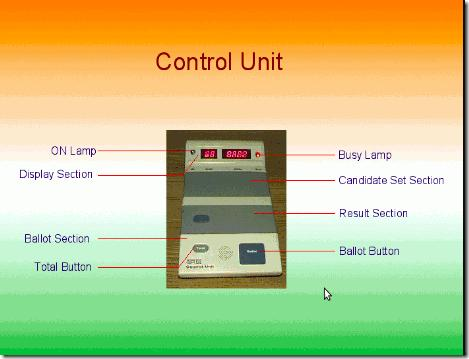
\includegraphics[width=0.7\textwidth]{evm-control-thumb1.jpg}}{0.7}
  \end{annotate}
  \caption{Control Unit\protect\footnotemark}\label{fig:Airbus}
\end{figure}


\subsection{Printer Unit}

\begin{figure}[h!]
  \centering
  \begin{annotate}{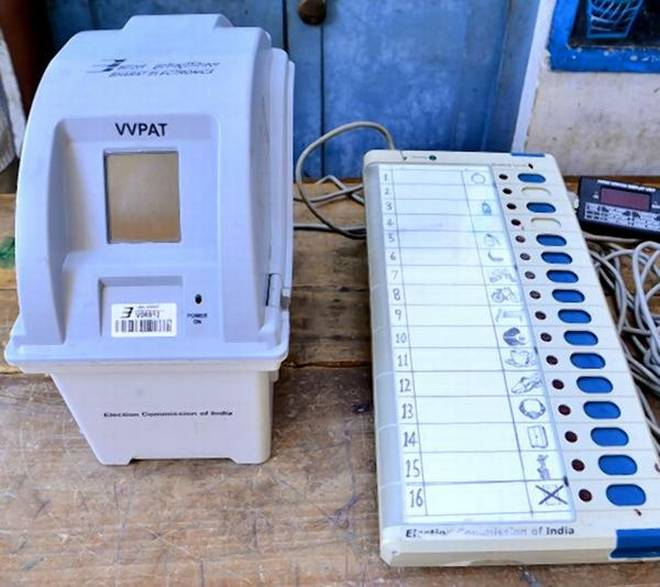
\includegraphics[width=0.6\textwidth]{vvpat.jpeg}}{0.7}
  \end{annotate}
  \caption{Printer Unit\protect\footnotemark}\label{fig:Airbus}
\end{figure}


This is a recent addition to the EVM system. When politicians in the country started crying foul that the EVMs are rigged and that no matter what button is pressed on the ballot all votes go to the party in power, etc. the VVPAT feature was introdcued. VVPAT stands for Voter Verified Paper Audit Trail. When a voter casts a vote on the ballot, the Printer Unit prints which candidate the voter voted for and displays it to the candidate for a brief amount of time before being stored in another box. These pieces of paper are tallied with the Control Unit results to ensure that there is no discrepancy between the actually cast votes and the counted votes. 

\section{State Diagram of System}

\begin{figure}[h!]
  \centering
  \begin{annotate}{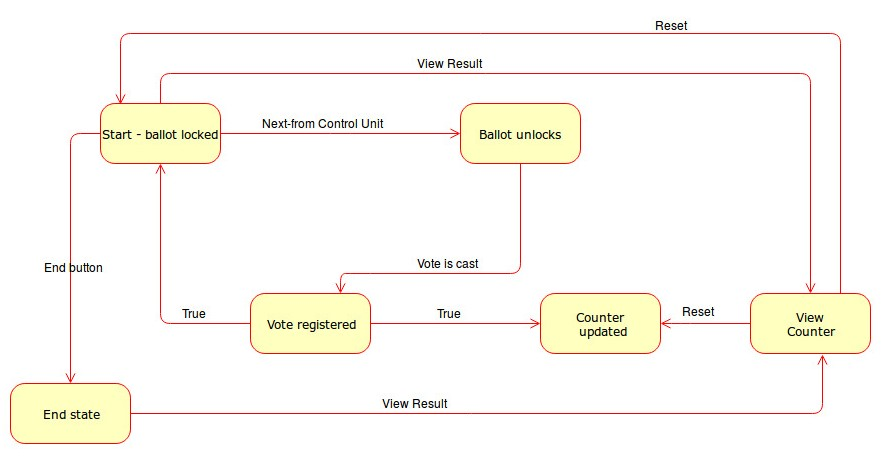
\includegraphics[width=1\textwidth]{state.jpg}}{0.8}
  \end{annotate}
  \caption{State diagram\protect\footnotemark}\label{fig:Airbus}
\end{figure}

\section{Problems with existing system:}
\begin{itemize}
    \item The final votes will be counted based on what is shown on the LCD display. It is easy to change the 7 segment display to manipulate the results by replacing it with a tampered unit. 
    
    \item The source code for the control and ballot units is unreadable and hence it leads to a suspicion of manufacturer rigging the system before hand.
    
    \item Mock elections are held to ensure the EVM's are working correctly, but since they are on a smaller scale it might be easy to incorporate a threshold on number of votes, only after which tampering occurs.
    
    \item Secure storage in strong rooms is also doubtful. There is ample time to tamper with the machines should someone get access to it.  
\end{itemize}

\section{Proposed solutions}
\begin{itemize}
    \item Improved Seals:
    \begin{itemize}
        \item The EVM can only be tampered with by contact. Since there is no use of the net anywhere there is no scope of online hacking. 
        \item Existing seals are very easy to break and replicate. Making them more solid and tamper proof will help reduce any chance of tampering.
        \item Solid metal seals with a self destruct or alarm feature is an option. Should someone try to open the seal or somehow manage to penetrate it, the source code should be able to identify the intrusion and self destruct or send an alarm. Or the display can be made to read tampered. 
        \item The current display is easily replaceable, it needs to be welded solid so it can't be changed or manipulated. 
    \end{itemize}
    
    \item Transparency in manufacturing:
    \begin{itemize}
        \item Since once the source code is burned onto the chip it cant be changed or even read, it is very important to make sure that the source code that is being burned onto the chip is correct and doesn't cause any manipulations. 
        \item This can be done by keeping a check on the manufacturing site, frequent and rigorous testing of the machines randomly, etc.
    \end{itemize}
    
    \item Testing the EVMs:
    \begin{itemize}
        \item EVMs need to be tested properly to make sure they are working correctly. They need to tested to their count limit and not only to a smaller value. 
        \item Democracy involves assuring people that they are part of a free, fair election. And if that involves a tedious step it needs to be taken. 
    \end{itemize}
    
    \item Change the entire protocol? Enter Blockchain
    \begin{itemize}
        \item With the rise of internet freedom and transparency which result in technologies like the Blockchain it is maybe time for the system to also adapt to it. 
        \item Blockchain by definition tries to solve the double-spending problem. Which is basically that the same currency can be spent twice if not checked. This is not good for the economy. Right now this is avoided by 3rd party institutions like banks and governments. Blockchain eliminates the need for a 3rd party by creating a peer to peer network and an open ledger of records. 
        \item Elections can also be thought of as a transaction problem, where each person has one vote and it needs to be transacted to one candidate only. There should not be any double spending. Right now this is being taken care of by a 3rd party, the Election Commission. 
        \item A peer to peer system can be created using the existing electoral college lists, where everyone can vote and no tampering will occur, solely based on the strength of the ledger. 
        \item The ledger is very secure because of encryptions happening after each valid transaction. Since it is decentralized, compromising the ledger would be close to impossible. 
        \item This however raises the question of the procedure in which elections are held. Creating a peer to peer network at the individual level will be difficult when it comes to illiterate people. So nodes in the network can be at the polling booth level, where everyone comes to vote as usual, but instead of the control unit recording their vote, the ledger will. This can be done because the number of people registered to a specific polling station is fixed and since only they will be voting, the issue of double votes wont arise. 
        \item Since the ledger is decentralized there is no question of transparency. Any miner (blockchain jargon) can now keep track of the ledger. 
        \item A crude visual depiction of the process (PCs = miners)
        \begin{figure}[h!]
          \centering
          \begin{annotate}{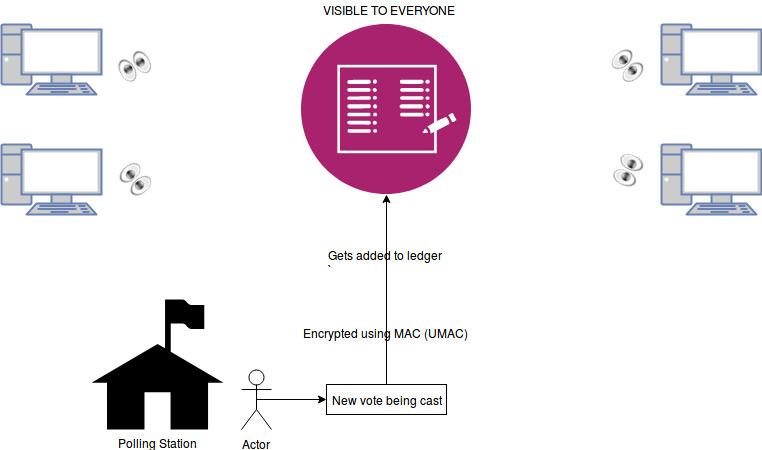
\includegraphics[width=0.8\textwidth]{blockchain_election.jpg}}{0.7}
          \end{annotate}
          \caption{Election using blockchain\protect\footnotemark}\label{fig:Airbus}
        \end{figure}
        \item Anonymity of the voters can still be maintained by using protocols such as WHISPER (followed by ethereum). And since a peer network is involved now the code which ensures the vote goes to an appropriate candidate can also be open sourced - something which was previously in closed. 
        \item UMAC is a message authentication code which is unbreakable and hence hackers influencing the vote at this level is also impossible. 
        \item There are yet a lot of technical details that have not been discussed and need more thought. But this seems to be a very promising avenue. To democratize elections using the most free software there is. 
    \end{itemize}
\end{itemize}

\section{Acknowledgements}
\begin{itemize}
    \item I would like to thank my partner (for the previous 2 assignments) and roommate, Kamalnath Polakam, 2015CS10244 for brainstorming with me, which led me to gain better clarity. 
    \item I would like to thank \href{draw.io} for their exceptionally convinient platform to draw charts and figures. All figures have been made using their website.
    \item I would also like to thank the internet.
\end{itemize}

\section{Bibliography}
\begin{itemize}
    \item \href{https://en.wikipedia.org/wiki/Blockchain}
    \item \href{https://en.wikipedia.org/wiki/UMAC}
    \item \href{https://en.wikipedia.org/wiki/Peer-to-peer}
    \item \href{https://bitcoin.org/bitcoin.pdf}
    \item \href{https://www.youtube.com/watch?v=vVsIHCTGjsE&list=PL2-dafEMk2A7RTBlSSKdnehec0zJO-xLZ}
    \item \href{https://www.youtube.com/watch?v=93E_GzvpMA0}
    
\end{itemize}


\end{document}